\chapter{Supplementary figures}
\label{app:figures}

\section{FTIR replicates}
\label{app:ftir}
This appendix gives FTIR data not included in the main text. Figure~\ref{fig:app_ftir_full} shows the full measured range (\qtyrange{400}{4000}{cm^{-1}}) of the mean spectra. The region below \qty{1000}{cm^{-1}} is dominated by polysulfone bands and shows no differences between conditions, and the region between 1800 and \qty{2800}{cm^{-1}} contains no bands; both were therefore left out of Figure~\ref{fig:ftir}. Figure~\ref{fig:app_ftir_scans} shows the three individual scans for each sample, which overlap closely.

\begin{figure}[htbp]
    \centering
    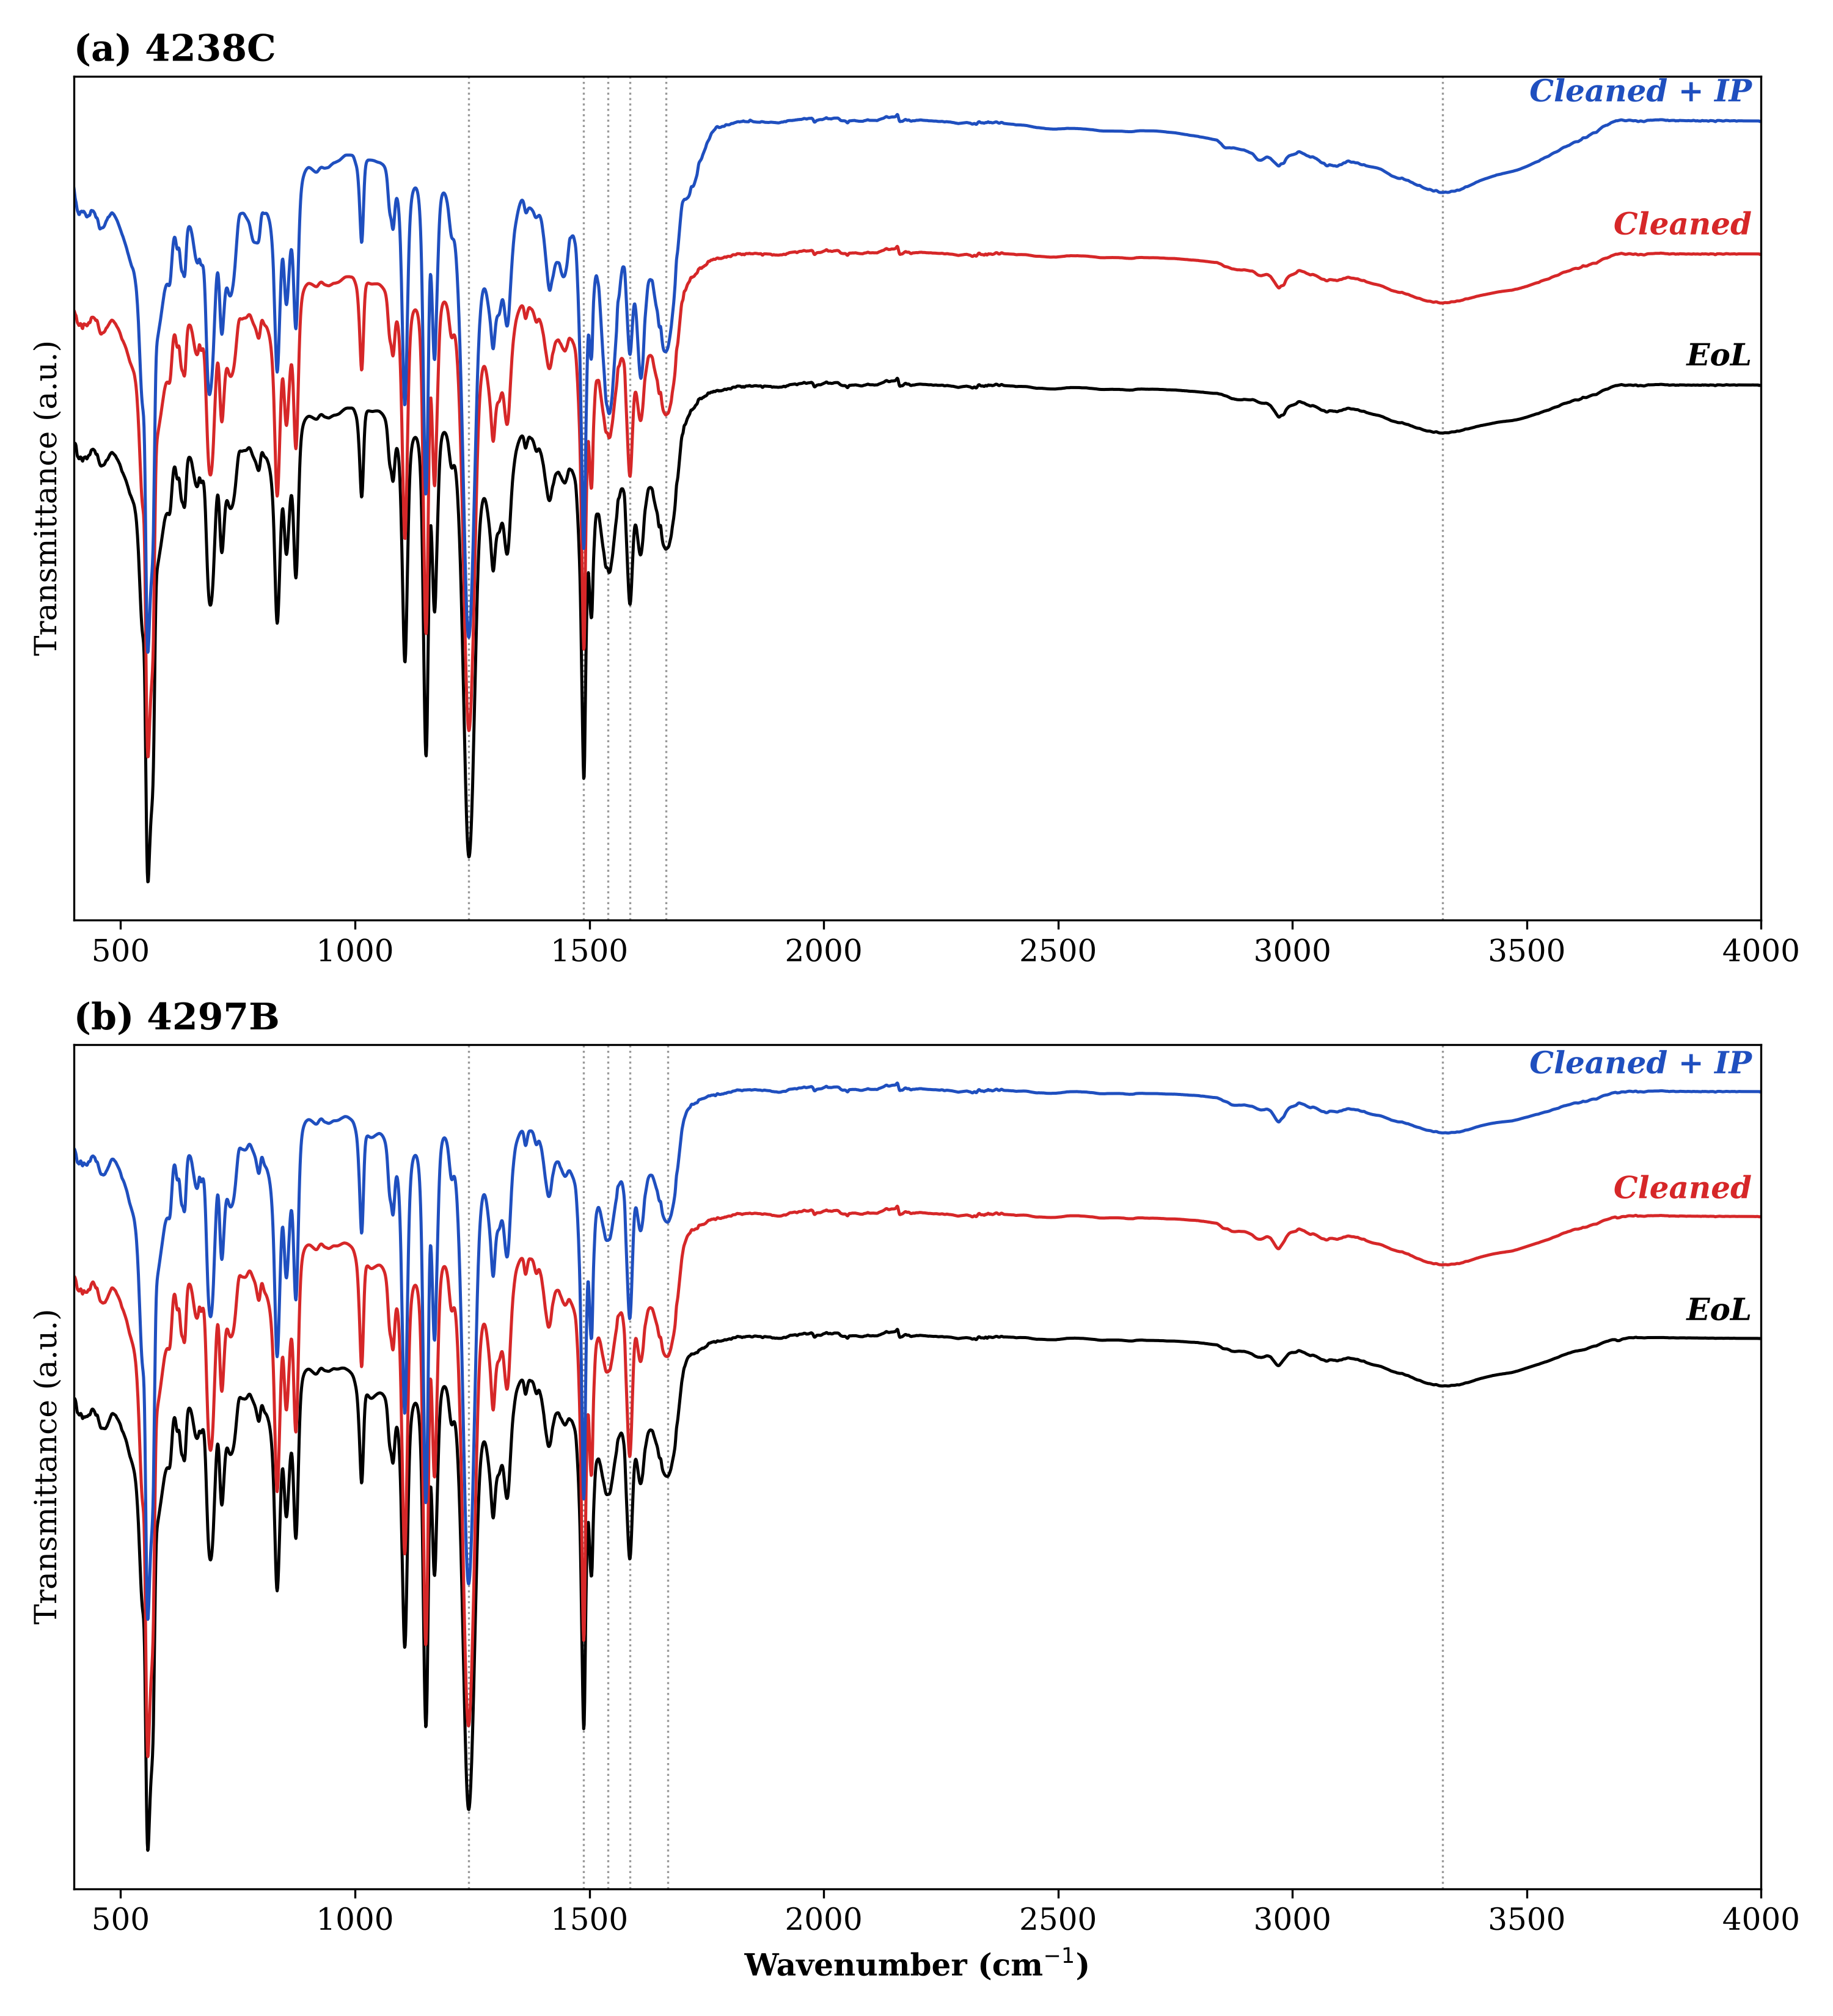
\includegraphics[width=0.5\textwidth]{figures/Analysis/FTIR/FTIR_full_spectra.png}
    \caption{Full-range ATR-FTIR spectra (mean of three scans) of EoL,
    extensive-clean and extensive-clean + IP coupons of (a) 4238C and
    (b) 4297B.}
    \label{fig:app_ftir_full}
\end{figure}

\begin{figure}[htbp]
    \centering
    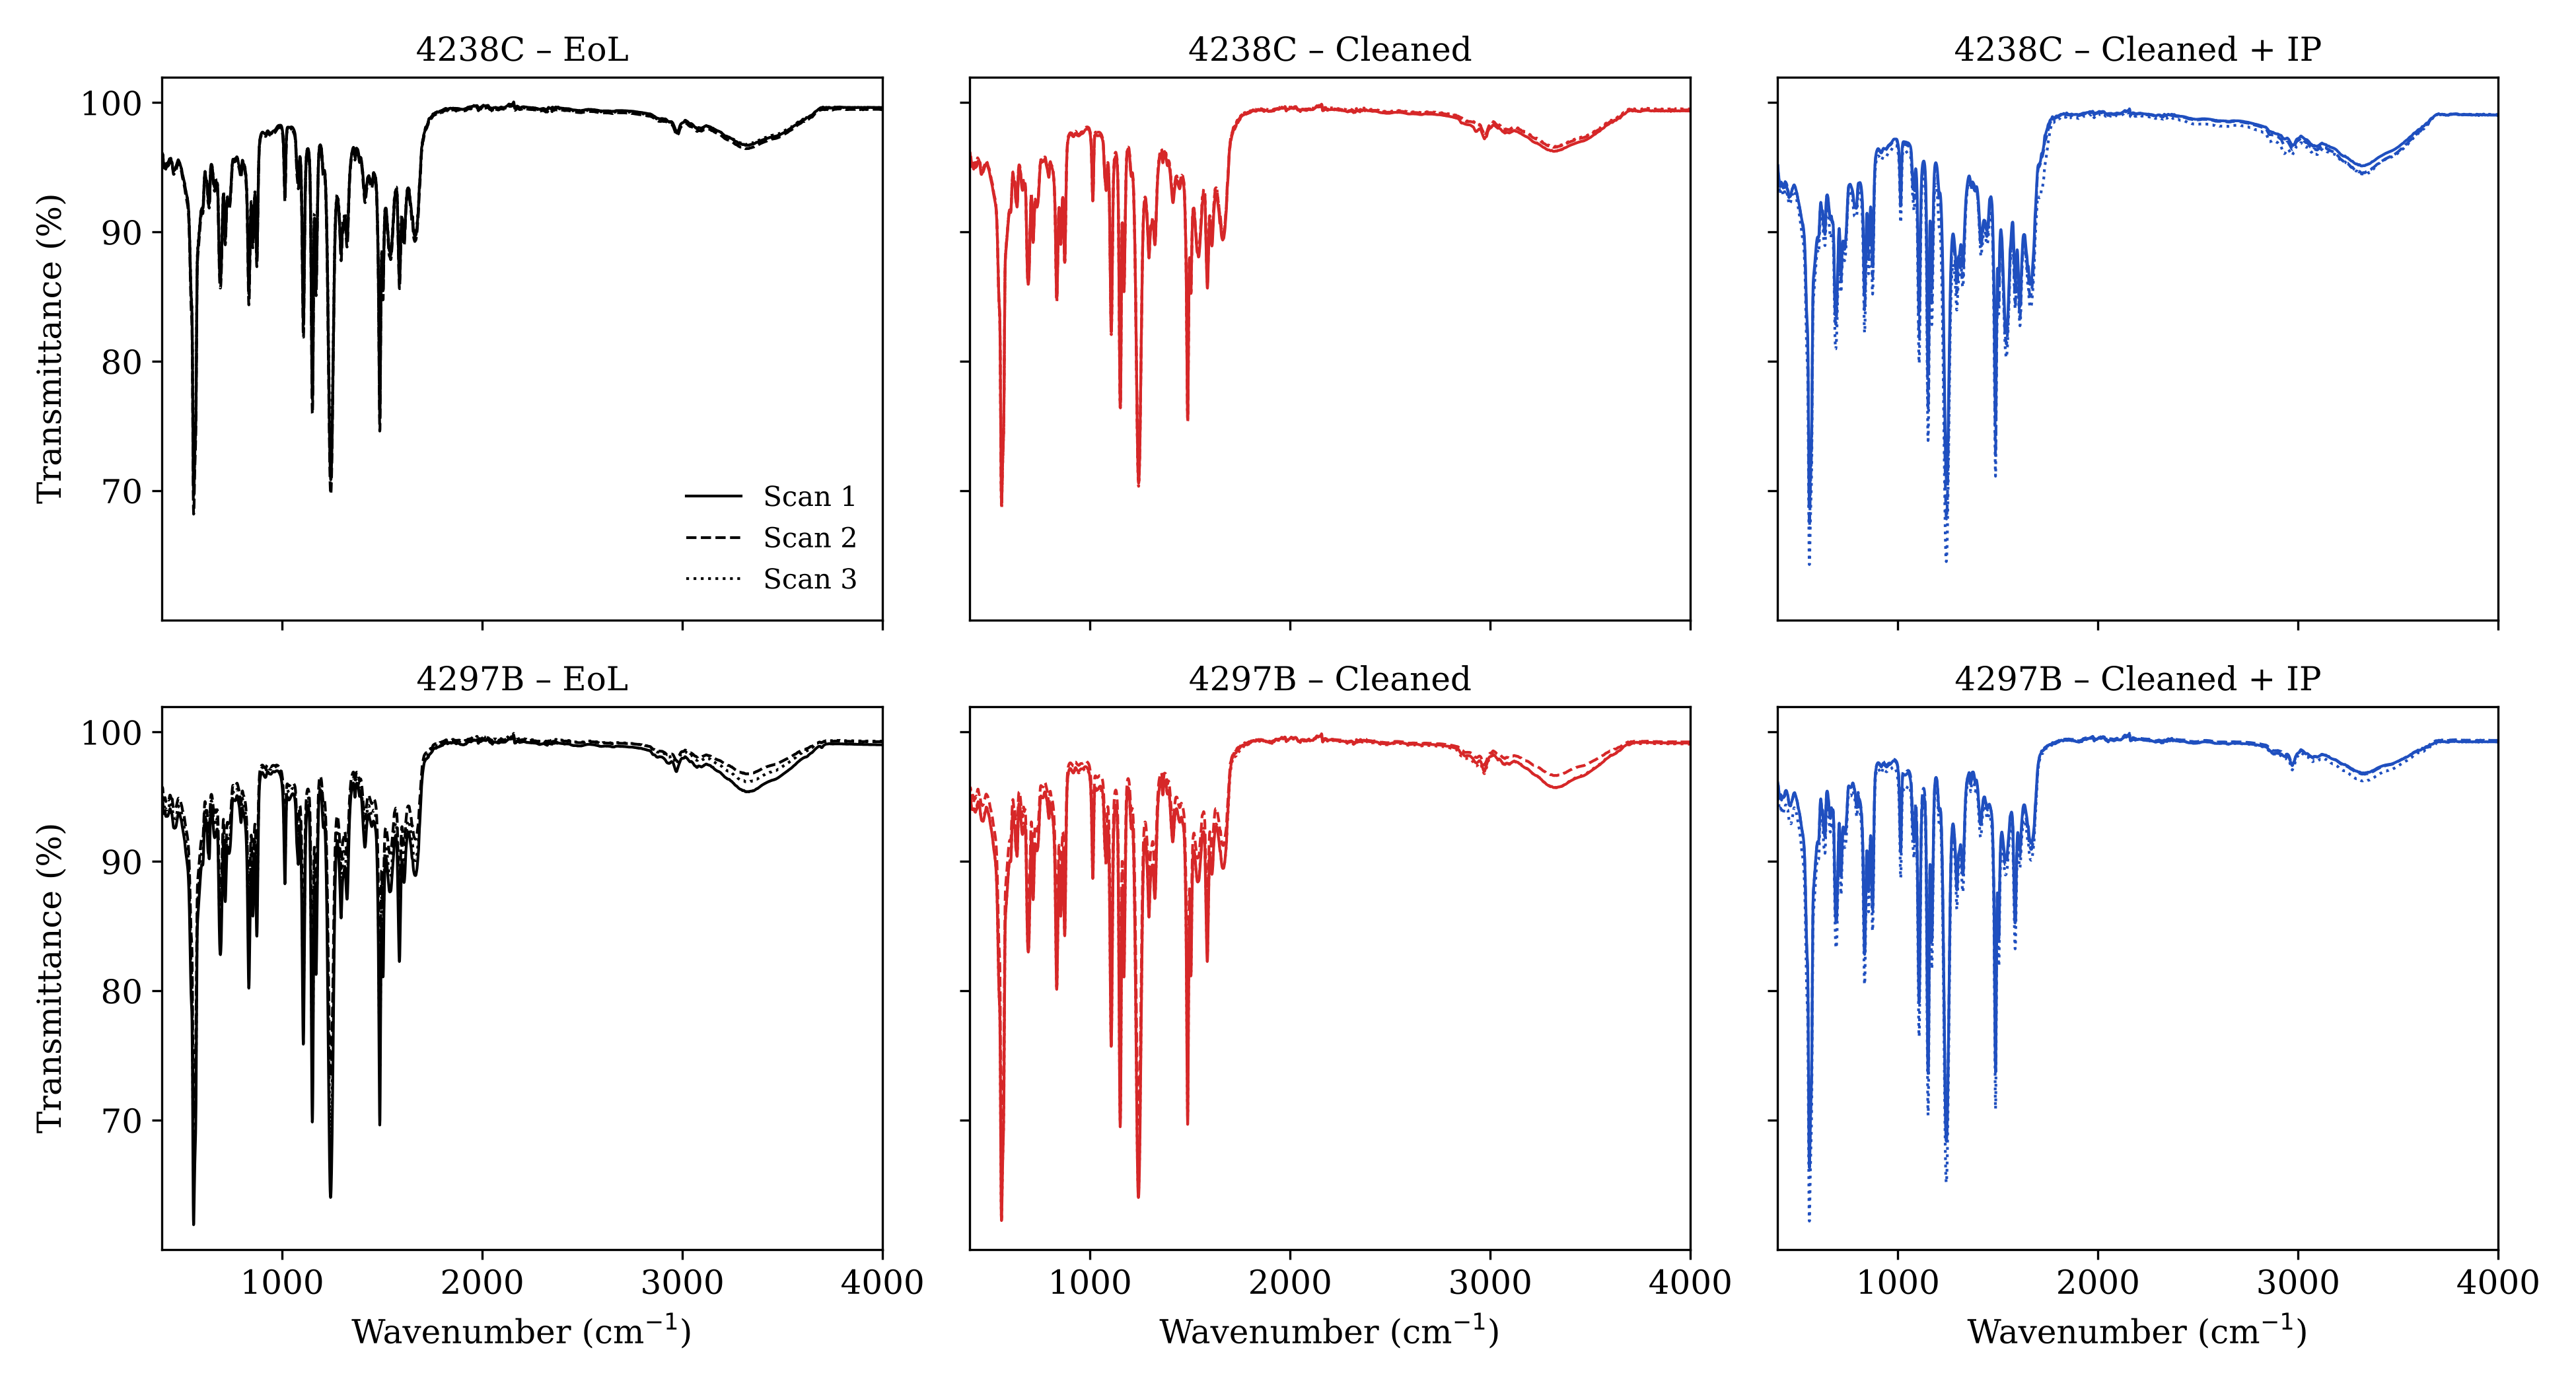
\includegraphics[width=\textwidth]{figures/Analysis/FTIR/FTIR_replicate_scans.png}
    \caption{Individual ATR-FTIR scans (three per sample) of each membrane and
    condition.}
    \label{fig:app_ftir_scans}
\end{figure}

\section{Additional SEM images}
\label{app:sem}
This section presents SEM images aquired during this thesis that were not included in the main text.  All images were taken on a Nova NanoSEM. The end-of-life 4238C images in Figure~\ref{fig:app_sem_4238C_eol} were acquired in a separate session using the through-lens detector (TLD) at 5~kV; all other images were acquired with the Everhart--Thornley detector (ETD) at 10~kV.

\paragraph{End-of-life 4238C}
Figure~\ref{fig:app_sem_4238C_eol} shows the as-received 4238C surface over larger fields of view than Figure~\ref{fig:sem_4238C_eol}. Across all three images, smooth film-like regions alternate with areas of exposed ridge-and-valley structure containing dark openings. This shows that the
damage to the PA layer discussed in Section~\ref{sec:res-fouling-4238C} is spread across the surface rather than confined to one area.

\begin{figure}[htbp]
    \centering
    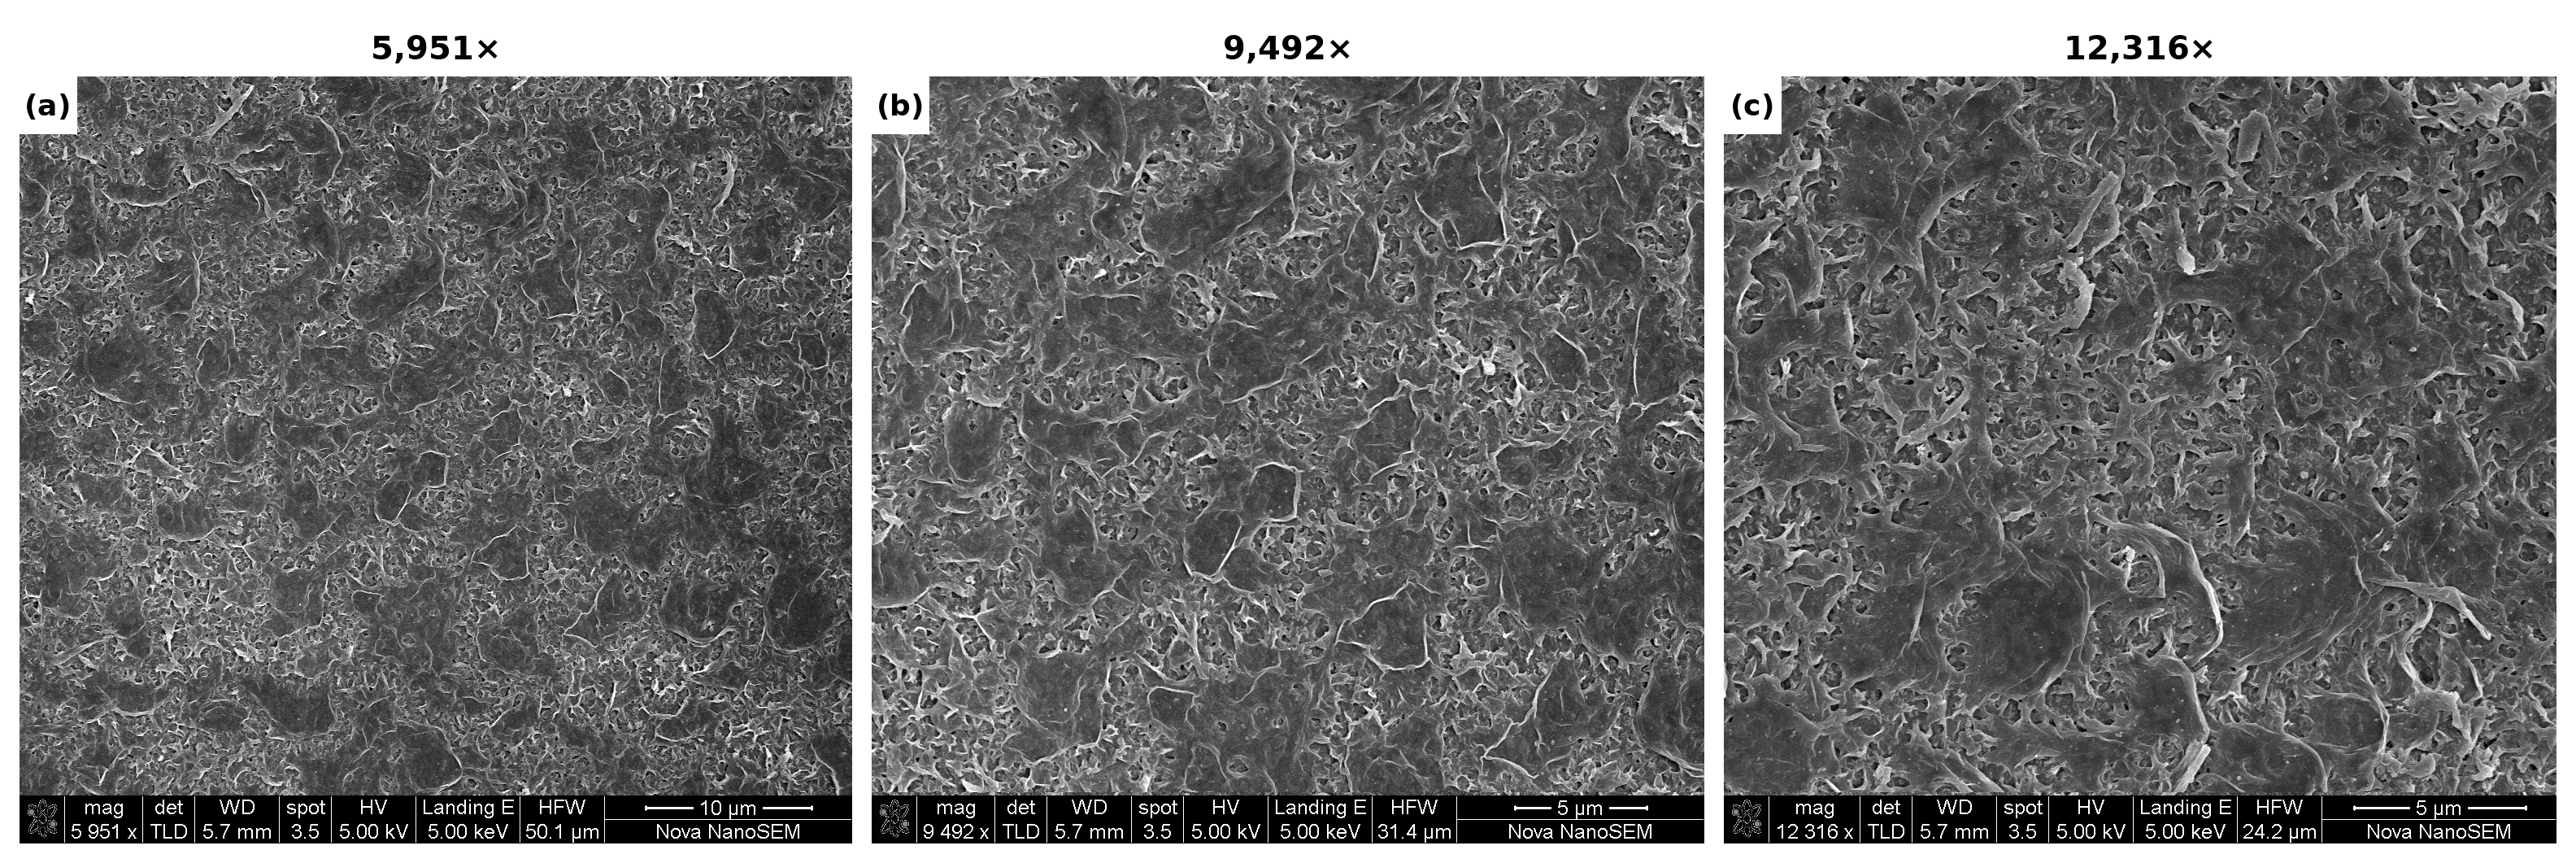
\includegraphics[width=\textwidth]{figures/Analysis/SEM/Unused/AppC_4238C_EoL_additional.png}
    \caption{Additional SEM micrographs of the end-of-life (as received) 4238C
    membrane surface at (a) 5,951$\times$, (b) 9,492$\times$ and
    (c) 12,316$\times$.}
    \label{fig:app_sem_4238C_eol}
\end{figure}

\paragraph{Cleaned + IP coupons at higher magnification.}
Figure~\ref{fig:app_sem_ip_highmag} shows the cleaned + IP coupons of both
membranes at higher magnification than in Figures~\ref{fig:sem_4238C_comparison} and~\ref{fig:sem_4297B}. The 4238C surface (Figure~\ref{fig:app_sem_ip_highmag}a) has a uniform ridge-and-valley PA structure with no visible openings or deposits. The 4297B surface (Figure~\ref{fig:app_sem_ip_highmag}b) has a less uniform structure, with clusters of fine particles still present on the surface after cleaning and IP.

\begin{figure}[htbp]
    \centering
    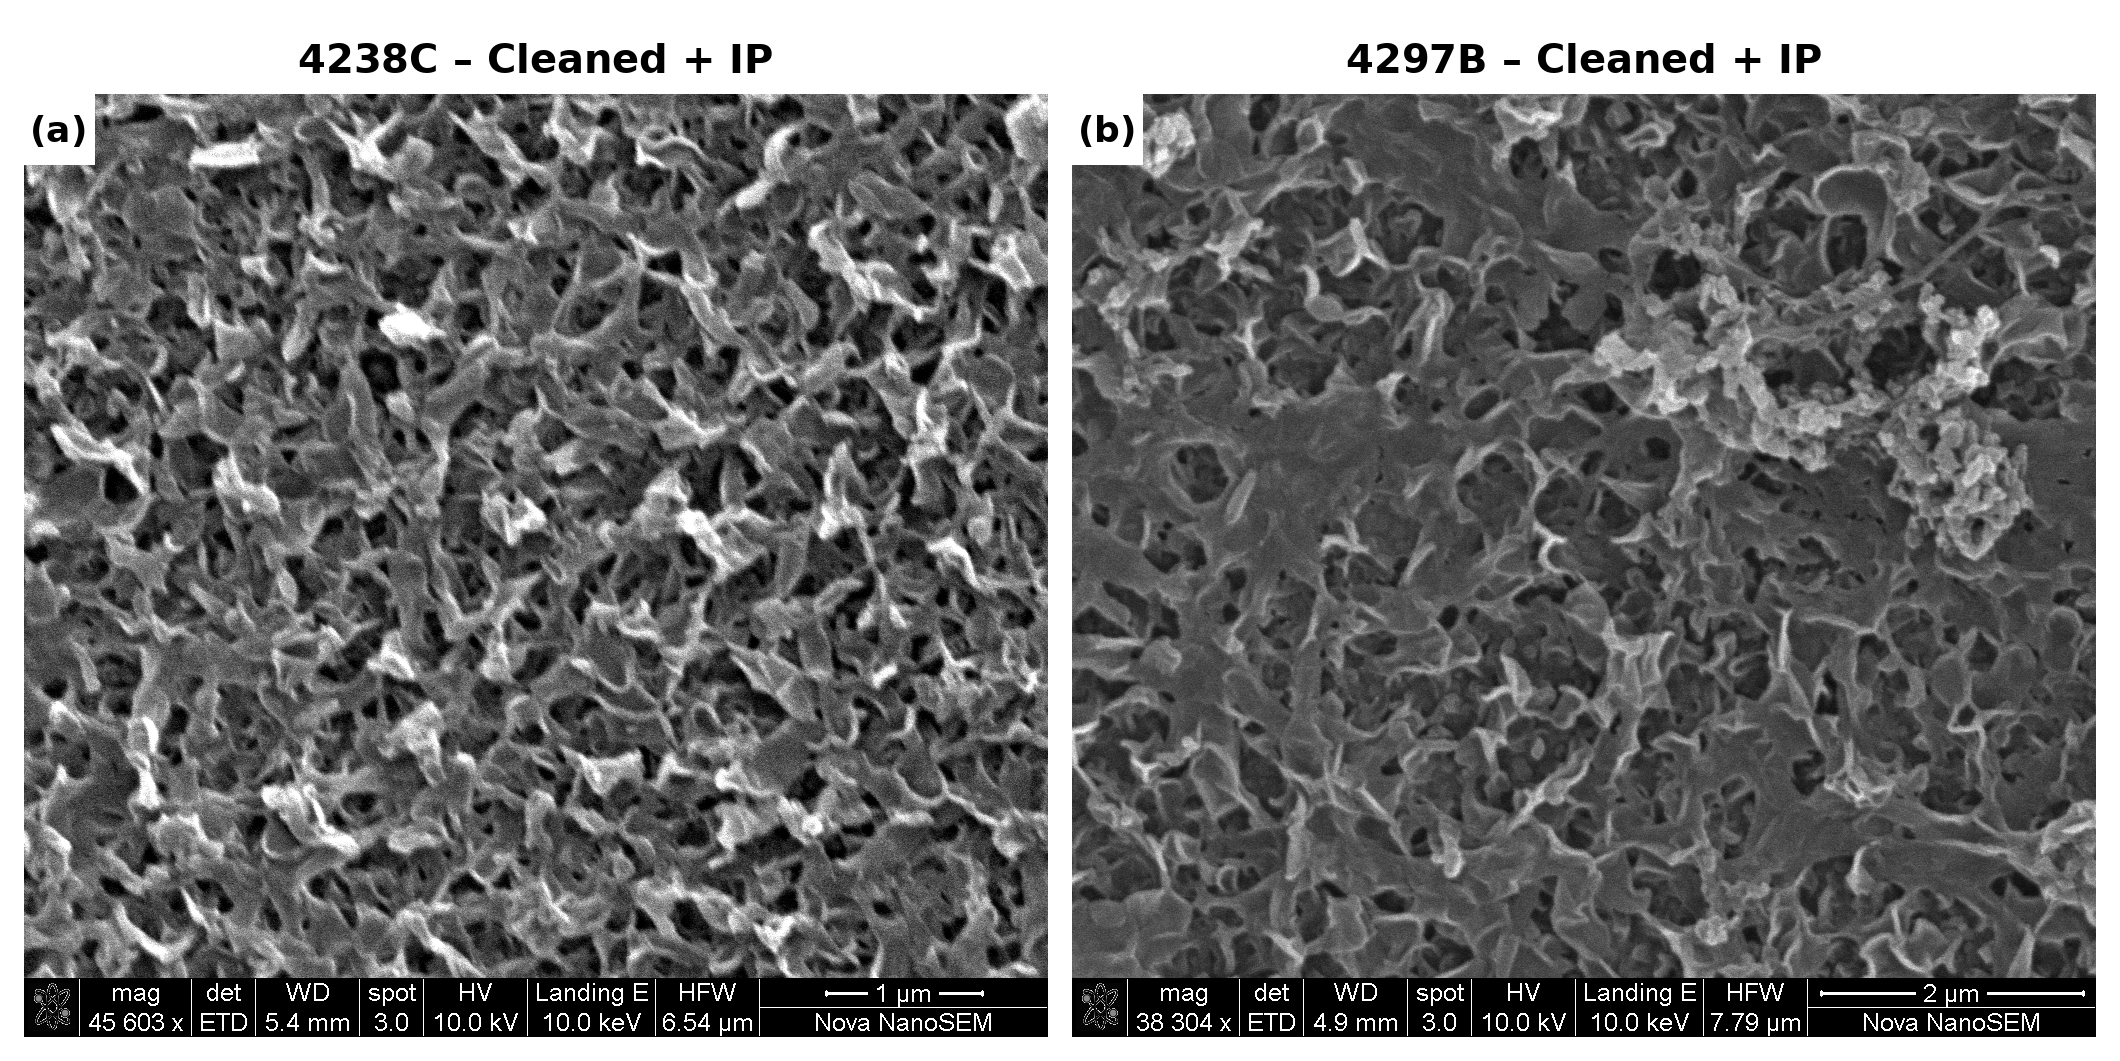
\includegraphics[width=0.67\textwidth]{figures/Analysis/SEM/Unused/AppC_CleanedIP_highmag.png}
    \caption{SEM micrographs of extensively cleaned + IP coupons at higher
    magnification: (a) 4238C (45,603$\times$) and (b) 4297B
    (38,304$\times$)}
    \label{fig:app_sem_ip_highmag}
\end{figure}
